\documentclass{article}
\usepackage{graphicx} % Required for inserting images
\usepackage{amsmath}
\usepackage{mathtools}
\usepackage{mathrsfs}
\usepackage{bbold}
\usepackage{hyperref}
\usepackage{bm}
\usepackage{comment}
\usepackage{here}
\usepackage{biblatex} %Imports biblatex package
\addbibresource{ref.bib} %Import the bibliography file


\title{Structural bounds for the sensitivity coefficients of non-linear chemical networks}
%\author{Simone Cavallero}
\date{\today}

\begin{document}
	
	\maketitle
	
	\section{Introduction}
	Recently, Horowitz, Owen \cite{1} and Esposito \cite{2} derived bounds on the sensitivity of chemical reaction networks (CRN), which characterize the response of the network to a perturbation of some of its kinetic parameters. Their results employed graph theory and linear algebra and for this reason are limited to linear CRNs. Inspired by these works, we explore here similar results for non-linear CRNs, in particular for autocatalytic CRNs. Our goal is to understand structural properties which depend on the stoichiometry or topology of a CRN but which are independent of the kinetics, because these properties are related to the robustness of the network.
	
	Recently, structural bounds for thermodynamic quantities have been derived for autocatalytic networks \cite{4} in the regime of maximal production of products, i.e. for a maximal output flux. The bounds we study here are of a different type, because they do not require the maximization of any flux in the system, nevertheless both bounds could be related since they are both structural in the sense defined above.
	
	In the literature, various groups have studied structural properties of chemical networks. For instance, G. Giordano et al. introduced the influence matrix, which quantifies how external inputs affect the sign of the steady-state outputs \cite{giordano_computing_2016}. Along these lines, Hirono et al. studied another structural property in which steady-state reaction fluxes in a network are invariant with respect to changes of parameters within a subnetwork, a property which they have called Robust Perfect Adaptation  \cite{5,6}. 
	
	\section{Simple illustrative example}
	Let us consider the type 1 autocatalytic network considered in \cite{4}, which is defined by :
	\begin{center}
		\begin{equation}
			\label{ex1}
			\begin{aligned}
				F+\alpha \mathrm{A} &\xrightleftharpoons[J_{-1}]{J_{+1}}\mathrm{B}\\
				\mathrm{B} &\xrightleftharpoons[J_{-2}]{J_{+2}}\beta \mathrm{A}+W,
			\end{aligned}
		\end{equation}
	\end{center}
	with $\alpha < \beta$ where $F$ and $W$ are respectively fuel and waste species. Lower case letters are used to denote concentrations of species, whether they are at steady state or not, while we use upper case letters to denote the species themselves. We assume $F$ and $W$ have a fixed concentrations, which can be incorporated in the rate constants.
	Let us also assume MAL kinetics :
	\begin{center}
		\begin{equation}
			\begin{aligned}
				J_1 &= k_1 a^{\alpha} - k_{-1} b \\
				J_2 &= k_2 b - k_{-2} a^{\beta}
			\end{aligned}
			\label{13}
		\end{equation}
	\end{center}
	
	When $A$ is chemostated in addition to $F$ and $W$, we have shown elsewhere that the system reaches a non-equilibrium steady state \cite{4}. In this non-equilibrium steady-state, the concentration $b=b(a)$ is obtained by solving $db/dt=J_1-J_2=0$, which leads to 
	\begin{center}
		\begin{equation}
			\label{b_SS}
			b= \frac{k_1 a^{\alpha}+k_{-2} a^{\beta}}{k_{-1}+k_2}.
		\end{equation}
	\end{center}
	From this, we deduce the logarithmic sensitivity coefficient, which quantifies the perturbation of the concentration of the variable species $B$ when $a$ is changed in this steady state  :
	\begin{center}
		\begin{equation}
			\label{eq:bound_A_chem}
			\frac{d\log b}{d \log a}= \frac{\alpha k_1 a^{\alpha}+\beta k_{-2} a^{\beta}}{k_{1} a^{\alpha}+k_{-2} a^{\beta}} \in [\alpha, \beta].
		\end{equation}
	\end{center}
	The important point is that this logarithmic sensitivity coefficient admits bounds in the non-equilibrium steady state of the system which depend on the stoichiometric coefficients $\alpha$ and $\beta$ but not on kinetic parameters $k_i$. In a way, one can interpret this logarithmic sensitivity coefficient as a kind of partial kinetic order of steady state concentration $b$ with respect to $a$.
	
	When instead $B$ is chemostated, the steady state concentration of $A$ is no longer an explicit function of $b$. In fact, the steady state condition $2 J_2 - J_1 =0$ defines an implicit function $a=a(b)$ difficult to invert. Nevertheless, we can still obtain the sensitivity coefficient from this implicit function :
	\begin{center}
		\begin{equation}
			\label{eq:bound_B_chem}
			\frac{d\log b}{d \log a}= \frac{\alpha^2 k_1 a^{\alpha}+\beta^2 k_{-2} a^{\beta}}{\alpha k_{1} a^{\alpha}+\beta k_{-2} a^{\beta}} \in [\alpha, \beta].
		\end{equation}
	\end{center}
	Although this coefficient is different from the one obtained in previous case where $A$ is chemostated, the same bound is obtained for this particular log-sensitivity coefficient.
	
	Note the importance of the assumption of MAL kinetics in these derivations (and similarly for our previous results \cite{4}), without it, the bounds on the sensitivity coefficients would not be only a function of stoichiometric coefficients. When this assumption is not made, one can still derive a weaker result concerning the sign of the sensitivity coefficient  \cite{giordano_computing_2016}. To show this, let us write the fluxes as $J_1=f_1(a)-f_{-1}(b)$ and $J_2=f_2(b)-f_{-2}(a)$, where the $f_i$ are positive and monotonous functions, which describe the non-MAL one way flux of reaction $i$. Then, when A is chemostated, the steady condition $J_1=J_2$ takes the form $f(a,b)=0$, with $f(a,b)=f_1(a)+f_{-2}(a)-f_{-1}(b)-f_{2}(b)$. It follows from this that 
	\begin{equation}
		\label{eq:bound_A_chem}
		\frac{d b}{d a}= -\frac{ \frac{\partial f}{\partial a} }{ \frac{\partial f}{\partial b} }= \frac{f'_1(a)+f'_{-2}(a)}{f'_{-1}(b)+f'_2(b)}.
	\end{equation}
	From the monotonicity of the functions $f_i$ follows the property that the coefficient $db/da$ is always positive (and therefore also the log-sensitivity coefficient $d \log b/ d \log a$), independently of kinetic parameters that may be needed to specify functions $f_i$. The same structural property for the sign of the sensitivity coefficient also holds when B is chemostated.
	
	\section{General framework}
	
	Here, we consider a general chemical reaction network described by with deterministic rate equations and we also do not make the assumption of MAL kinetics. Instead, we assume that this chemical network admits a well-defined steady-state, and we investigate how this steady-state is modified when some parameters in the network are changed. This question is very much the focus of metabolic control analysis (MCA) \cite{3}.
	
	Let us assume that the evolution equation of the concentration vector is $\textbf{x}= (x_1,x_2,...,x_n)^T$ is :
	\begin{center}
		\begin{equation}
			\frac{d\textbf{x}}{dt} = S \cdot \textbf{J},
		\end{equation}
	\end{center}
	with $S$ the $n \times r$ stoichiometric matrix and $\textbf{J}$ the vector of $r$ reaction rates. The steady state reads $S \cdot \textbf{J} = \textbf{0}$.
	
	The rates $\textbf{J}$ are now assumed to depend on an external parameter $\kappa$ which quantifies the perturbation. This parameter could be for instance a rate constant or a chemostated species. Then,
	\begin{center}
		\begin{equation}
			S\cdot \frac{d\mathbf{J}}{d\kappa} = \mathbf{0} \ \ \implies \ \ S \cdot \mathbf{J}_{\kappa} + S \cdot {\mathbb{J}}_{\mathbf{x}} \cdot \mathbf{x}_{\kappa} = 0
		\end{equation}
	\end{center}
	where
	\begin{center}
		\begin{equation}
			\mathbf{J}_{\kappa}= \left(\frac{d J_1}{d\kappa},...,\frac{d J_n}{d\kappa}\right)^T \ {\rm and} \ \ \
			{\mathbb{J}}_{\mathbf{x}}^{i,j} = \frac{d J_i}{d x_j}. 
		\end{equation}
	\end{center}
	
	This gives
	
	\begin{center}
		\begin{equation}
			S \cdot {\mathbb{J}}_{\mathbf{x}} \cdot \mathbf{x}_{\kappa} = - S \cdot \mathbf{J}_{\kappa}.
		\end{equation}
	\end{center}
	
	A key object is therefore the Jacobian matrix, which is the $n \times n$ square matrix $\mathbf{M} \coloneqq S \cdot \mathbb{J}_{\mathbf{x}}$.
	When this matrix is invertible, one obtains 
	an explicit expression for 
	the derivatives of the concentrations :
	\begin{center}
		\begin{equation}
			\mathbf{x}_{\kappa} = - \mathbf{M} ^ {-1} \cdot S \cdot \mathbf{J}_{\kappa}.
			\label{11}
		\end{equation}
	\end{center}
	Note that if we could further assume that $S$ and ${\mathbb{J}}_{\mathbf{x}}$ were both invertible, the inversion of the matrix $\mathbf{M}$ would be trivial, and
	the solution would be
	$\mathbf{x}_{\kappa} =  {\mathbb{J}}_{\mathbf{x}}^ {-1} \cdot \mathbf{J}_{\kappa}$. Unfortunately, this case rarely happens in practice, and we need to use Eq. \eqref{11}.
	
	In the MCA framework detailed in appendix A, the Jacobian is usually written as:
	\begin{center}
		\begin{equation}
			\mathbf{M}\coloneqq \mathbf{S_R} \cdot \bm{\Bar{\epsilon}_x} \cdot \mathbf{L}.
		\end{equation}
	\end{center}
	This is equivalent to the matrix introduced above because in our example there was no conservation laws. As a result, the link matrix is $\mathbf{L}= \mathbf{I}$ and $\mathbf{S_R}= \mathbf{S}$. Note that  $\mathbb{J}_{\mathbf{x}}$ is called elasticity matrix $\bm{\Bar{\epsilon}_x}$ in MCA theory. 
	
	The main difference is that  $\bm{\bar{\epsilon}}_{\pmb{\kappa}}$ involves perturbations with respect to many parameters $\pmb{\kappa}$, whereas $\mathbf{J}_{\kappa}$ is a vector of derivatives with respect to a single parameter $\kappa$. 
	
	From Eq. \eqref{11}, one deduces the sensitivity coefficients, which are log-derivatives of the concentrations, provided the steady-state vector $\mathbf{x}$ itself is known. In principle, we would like to obtain bounds on these sensitivity coefficients using Eq. \eqref{11} but without having to know the steady-state explicitly.
	
	
	\section{Illustrative examples}
	
	\subsection{Perturbation with respect to a metabolite concentration
	}
	Let us apply this general framework to the previous example.
	When $A$ is chemostated, the vector $\mathbf{x}$ only contains species $b$, $\mathbf{x}=b$, and the parameter with respect to which we are perturbing the system is the concentration $a$, thus $\kappa=a$.
	Then :
	\begin{center}
		\begin{equation}
			\begin{aligned}
				S = \begin{pmatrix}
					1 & -1
				\end{pmatrix}, \ \ \ \ \
				\textbf{J}_a =  \begin{pmatrix}
					\frac{d J_1}{d a} \\ \\
					\frac{d J_2}{d a}
				\end{pmatrix}, \ \ \ \ \
				\mathbb{J}_{b} = \begin{pmatrix}
					\frac{d J_1}{d b} \\ \\
					\frac{d J_2}{d b}.
				\end{pmatrix} \ \ \ \ \
			\end{aligned}
			\label{14}
		\end{equation}
	\end{center}
	
	Note that $S$ and $\mathbb{J}_{b}$ are not invertible, but their product is, since
	$S \cdot \mathbb{J}_{b} = - (k_2 + k_{-1})$.
	Thus, exploiting \eqref{11}, we get:
	\begin{center}
		\begin{equation}
			\frac{d b}{d a} = - \left( S \cdot {\mathbb{J}}_{b} \right)^ {-1} \cdot S \cdot \mathbf{J}_{a} = \frac{\alpha k_1 a^{\alpha-1}+\beta k_{-2} a^{\beta-1}}{k_{-1}+k_2}
		\end{equation}
	\end{center}
	We deduce from this, the log-sensitivity coefficient :
	\begin{center}
		\begin{equation}
			\frac{d \log b}{d \log a} = \frac{\alpha k_1 a^{\alpha}+\beta k_{-2} a^{\beta}}{(k_{-1}+k_2) b}.
		\end{equation}
	\end{center}
	Now using the steady-state concentration $b=b(a)$ from Eq. \ref{b_SS}, we recover the expression for the log-sensitivity coefficient $d\log b/d \log a$ of \eqref{eq:bound_A_chem}.
	
	
	When $B$ is chemostated, the situation is very similar, with $\mathbf{x}=a$ and $\kappa = b$. Now, the relevant matrix and vectors are  :
	\begin{center}
		\begin{equation}
			\begin{aligned}
				S = \begin{pmatrix}
					-\alpha & \beta
				\end{pmatrix}, \ \ \ \ \
				\textbf{J}_b =  \begin{pmatrix}
					-k_{-1} \\ \\
					k_2
				\end{pmatrix}, \ \ \ \ \
				\mathbb{J}_{a} = \begin{pmatrix}
					\alpha k_1 a^{\alpha-1} \\ \\
					-\beta k_{-2} a^{\beta-1}
				\end{pmatrix} \ \ \ \ \
				\label{19}
			\end{aligned}
		\end{equation}
	\end{center}
	
	Then, exploiting \eqref{11} we get
	\begin{center}
		\begin{equation}
			\frac{d a}{d b} = - \left( S \cdot {\mathbb{J}}_{a} \right)^ {-1} \cdot S \cdot \mathbf{J}_{b} = \frac{\alpha k_{-1}+\beta k_2}{\alpha^2 k_1 a^{\alpha-1}+\beta^2 k_{-2} a^{\beta-1}},
		\end{equation}
	\end{center}
	and the log-sensitivity reads:
	\begin{center}
		\begin{equation}
			\frac{d \log a}{d \log b} = b \frac{\alpha k_{-1}+\beta k_2}{\alpha^2 k_1 a^{\alpha}+\beta^2 k_{-2} a^{\beta}}.
		\end{equation}
	\end{center}
	
	Now using the implicit expression $b=b(a)$ derived from the steady state equation, we immediately recover the log-sensitivity coefficient of Eq. \eqref{eq:bound_B_chem}.
	
	
	
	
	
	
	\section{Response to perturbations with respect to rate constants}
	
	Now, let us consider that the perturbation concerns kinetic parameters such as rate constants.
	
	\subsection{Sensitivities of type I autocatalytic core}
	Let us consider again the example of Eq. \ref{ex1}. We still assume that three species are chemostatted $F$, $W$ and $A$ or $B$, so that the system reaches a non-equilibrium steady state.
	
	\subsubsection{A chemostated}
	The steady state is still given by Eq. \ref{b_SS} and 
	the matrices $S$ and $\mathbb{J}_b$ are unchanged with respect to the previous case. The only new matrices are 
	
	\begin{center}
		\begin{equation}
			\mathbf{J}_{k_1} = \begin{pmatrix}
				\frac{d J_1}{d k_1} \\ \\
				\frac{d J_2}{d k_1}
			\end{pmatrix}= \begin{pmatrix}
				a^{\alpha} \\ \\
				0
			\end{pmatrix}
			\label{53}
		\end{equation}
	\end{center}
	
	then, from \eqref{11}
	
	\begin{center}
		\begin{equation}
			\frac{d b}{d k_1} = - \left( S \cdot {\mathbb{J}}_{b} \right)^ {-1} \cdot S \cdot \mathbf{J}_{k_1} = \frac{a^{\alpha}}{k_{-1}+k_2}
		\end{equation}
	\end{center}
	
	leading to
	
	\begin{center}
		\begin{equation}
			\frac{d \log b}{d \log k_1} =  \frac{k_1 a^{\alpha}}{(k_{-1}+k_2)b_{ss}} = \frac{k_1 a^{\alpha}}{k_{1}a^{\alpha}+k_{-2}a^{\beta}}
		\end{equation}
	\end{center}
	
	giving
	
	\begin{center}
		\begin{equation}
			\frac{d \log b}{d \log k_1} \in \left[0,1\right]
		\end{equation}
	\end{center}
	
	\begin{comment}
		Perturbing $k_2$ instead, what changes is just
		
		\begin{center}
			\begin{equation}
				\mathbf{J}_{k_2} = \begin{pmatrix}
					\frac{d J_1}{d k_2} \\ \\
					\frac{d J_2}{d k_2}
				\end{pmatrix}= \begin{pmatrix}
					0 \\ \\
					b
				\end{pmatrix}
				\label{57}
			\end{equation}
		\end{center}
		
		Then, from \eqref{11}:
		
		\begin{center}
			\begin{equation}
				\frac{d b}{d k_2} = - \left( S \cdot {\mathbb{J}}_{b} \right)^ {-1} \cdot S \cdot \mathbf{J}_{k_2} = -\frac{b}{k_{-1}+k_2}
			\end{equation}
		\end{center}
	\end{comment}
	
	One can then use the same framework to compute the cases for the other rate constants, just changing $\mathbf{J}_{\kappa}$. One obtains:
	
	\begin{center}
		\begin{equation}
			\frac{d \log b}{d \log k_2} = \frac{k_2}{b} \frac{d b}{d k_2} = -\frac{k_2}{k_{-1}+k_2} \in \left[-1,0 \right]
		\end{equation}
	\end{center}
	\begin{comment}
		Perturbing $k_{-1}$, what changes is just
		
		\begin{center}
			\begin{equation}
				\mathbf{J}_{k_{-1}} = \begin{pmatrix}
					\frac{d J_1}{d k_{-1}} \\ \\
					\frac{d J_2}{d k_{-1}}
				\end{pmatrix}= \begin{pmatrix}
					-b \\ \\
					0
				\end{pmatrix}
				\label{60}
			\end{equation}
		\end{center}
		
		Then
		
		\begin{center}
			\begin{equation}
				\frac{d b}{d k_{-1}} = - \left( S \cdot {\mathbb{J}}_{b} \right)^ {-1} \cdot S \cdot \mathbf{J}_{k_{-1}} = -\frac{b}{k_{-1}+k_2}
			\end{equation}
		\end{center}
		
		Then
	\end{comment}
	
	\begin{center}
		\begin{equation}
			\frac{d \log b}{d \log k_{-1}} = \frac{k_{-1}}{k_2} \frac{d \log b}{d \log k_2} \in \left[-1,0 \right]
		\end{equation}
	\end{center}
	
	\begin{comment}
		Lastly, perturbing $k_{-2}$
		
		\begin{center}
			\begin{equation}
				\mathbf{J}_{k_{-2}} = \begin{pmatrix}
					\frac{d J_1}{d k_{-2}} \\ \\
					\frac{d J_2}{d k_{-2}}
				\end{pmatrix}= \begin{pmatrix}
					0 \\ \\
					-a^{\beta}
				\end{pmatrix}
				\label{63}
			\end{equation}
		\end{center}
		
		\begin{center}
			\begin{equation}
				\frac{d b}{d k_{-2}} = - \left( S \cdot {\mathbb{J}}_{b} \right)^ {-1} \cdot S \cdot \mathbf{J}_{k_{-2}} = \frac{a^{\beta}}{k_{-1}+k_2}
			\end{equation}
		\end{center}
		
		Then
		
	\end{comment}
	
	\begin{center}
		\begin{equation}
			\frac{d \log b}{d \log k_{-2}} = \frac{k_{-2}}{b} \frac{d b}{d k_{-2}}=\frac{k_{-2}a^{\beta}}{k_1 a^{\alpha}+k_{-2} a^{\beta}} \in \left[0,1 \right]
		\end{equation}
	\end{center}
	
	\begin{figure}[H]
		\centering
		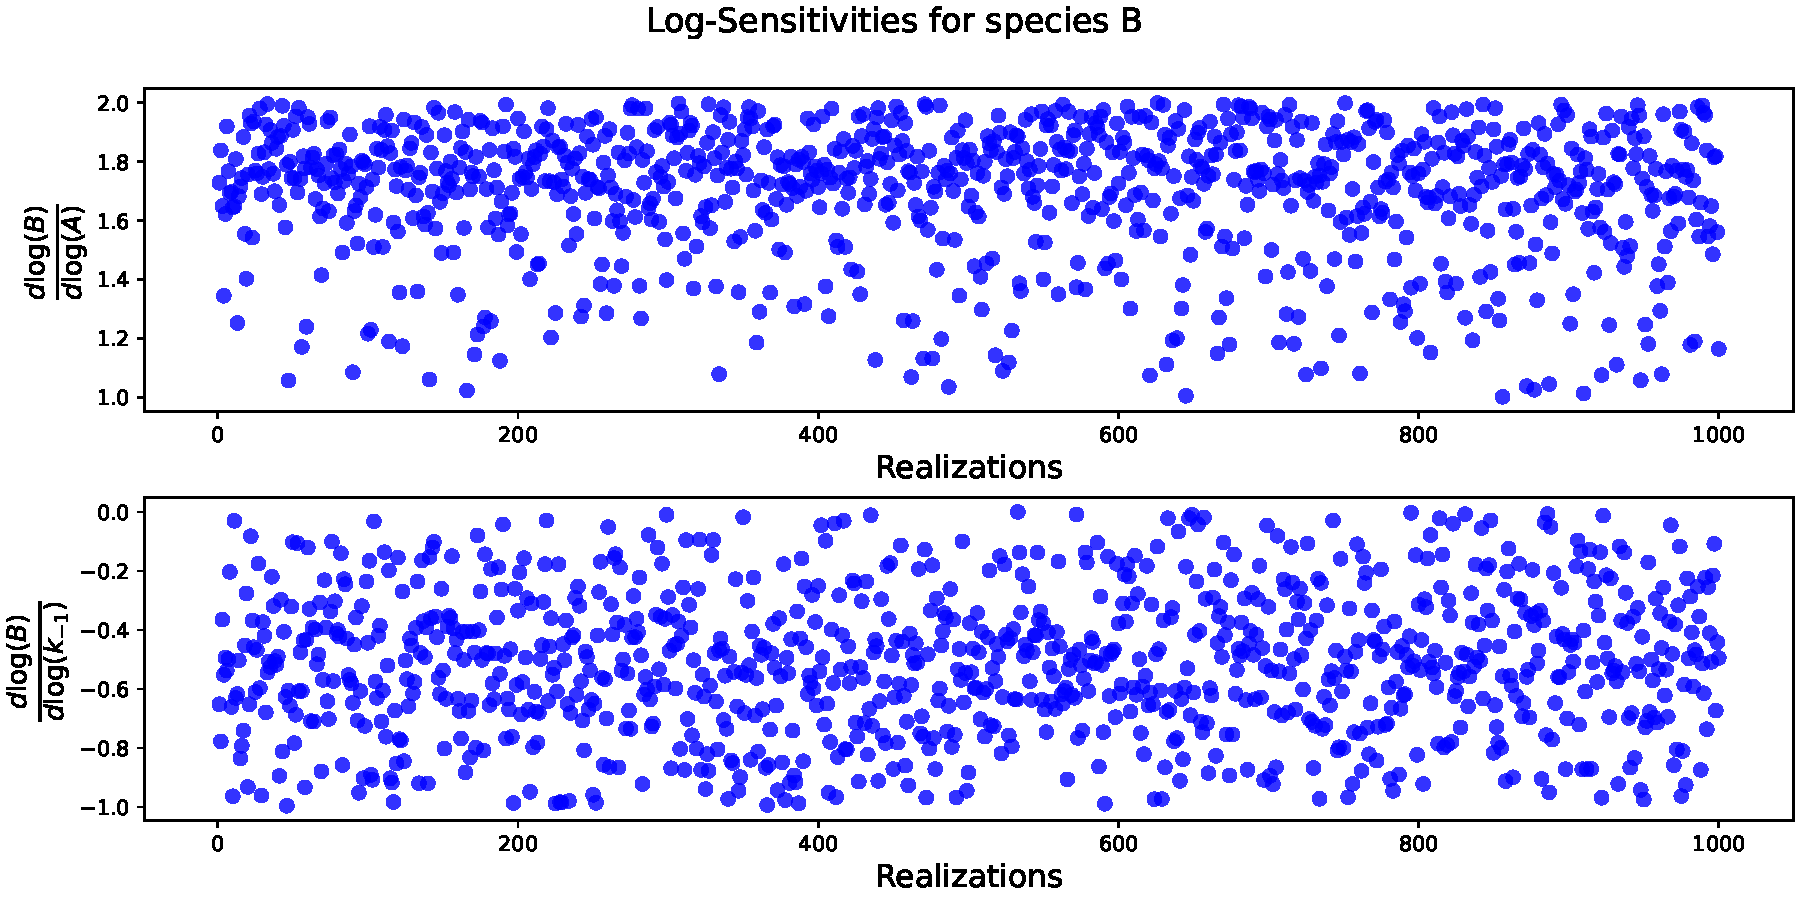
\includegraphics[width=1 \linewidth]{Sens_type1_chemoX1.pdf}
		\caption{\small{Numerical simulation for Type 1, with $\alpha = 1$ and $\beta = 2$ with 1000 realizations, randomized forward rate constants and $\boldsymbol{\mu_0}$: backward rate constants are constrained by thermodynamics. The results are only shown for perturbation on the chemostat and on $k_{-1}$. Log-sensitivities correctly follow the analytically predicted bounds, for A chemostated.}}
		\label{Fig. 1}
	\end{figure}
	
	\subsubsection{B chemostated}
	When $B$ is chemostated, calculations become a bit more subtle, because the steady state $a=a(b)$ is only implicitly defined from the equation :
	$$b=\frac{\alpha k_1 a^{\alpha}+\beta k_{-2} a^{\beta}}{\alpha k_{-1}+\beta k_2}.$$
	Note that
	$\mathbf{J}_{k_1}$, $\mathbf{J}_{k_2}$, $\mathbf{J}_{k_{-1}}$, $\mathbf{J}_{k_{-2}}$ will be respectively the same as what calculated for the case of $A$ chemostated, since they don't depend on the chemostat. This means that, perturbing $k_1$, following equation \eqref{11}, since $S\cdot \mathbf{J}_{k_1}=-\alpha a^{\alpha}$
	
	\begin{center}
		\begin{equation}
			\frac{d a}{d k_1} = - \left( S \cdot {\mathbb{J}}_{a} \right)^ {-1} \cdot S \cdot \mathbf{J}_{k_1} = -\frac{\alpha a^{\alpha}}{\alpha^2 k_1 a^{\alpha-1}+\beta^2 k_{-2}a^{\beta-1}}
		\end{equation}
	\end{center}
	
	Then 
	\begin{center}
		\begin{equation}
			\frac{d \log a}{d \log k_1} = \frac{k_1}{a} \frac{d a}{d k_1} = -\frac{\alpha k_1 a^{\alpha}}{\alpha^2 k_1 a^{\alpha}+\beta^2 k_{-2}a^{\beta}} \in \left[-\frac{1}{\alpha},0\right]
		\end{equation}
	\end{center}
	
	Perturbing $k_2$, we have that $S\cdot \mathbf{J}_{k_2}=\beta b$, so
	
	\begin{center}
		\begin{equation}
			\frac{d a}{d k_2} = - \left( S \cdot {\mathbb{J}}_{a} \right)^ {-1} \cdot S \cdot \mathbf{J}_{k_2} = \frac{\beta b}{\alpha^2 k_1 a^{\alpha-1}+\beta^2 k_{-2}a^{\beta-1}}
		\end{equation}
	\end{center}
	
	which means
	
	\begin{center}
		\begin{equation}
			\frac{d \log a}{d \log k_2} = \frac{\beta k_2 b}{\alpha^2 k_1 a^{\alpha}+\beta^2 k_{-2}a^{\beta}}
		\end{equation}
	\end{center}
	
	and substituting $b$
	
	\begin{center}
		\begin{equation}
			\frac{d \log a}{d \log k_2} =\frac{\beta k_2}{\beta k_2 + \alpha k_{-1}}\left( \frac{\alpha k_1 a^{\alpha}}{\alpha^2 k_1 a^{\alpha}+\beta^2 k_{-2} a^{\beta}}+\frac{\beta k_2 a^{\beta}}{\alpha^2 k_1 a^{\alpha}+\beta^2 k_{-2} a^{\beta}}\right)
			\label{70}
		\end{equation}
	\end{center}
	
	Now, the term outside the brackets lies in $\left[0,1 \right]$, the two terms inside instead lie respectively in $\left[0,\frac{1}{\alpha}\right]$ and in $\left[0,\frac{1}{\beta}\right]$ but when one term reaches 0, the other reaches for sure the maximum value, and being $\alpha < \beta$, what's inside the brackets must lie in the interval $\left[0, \frac{1}{\alpha} \right]$. This means that, overall 
	
	\begin{center}
		\begin{equation}
			\frac{d \log a}{d \log k_2} \in \left[0, \frac{1}{\alpha} \right]
		\end{equation}
	\end{center}
	
	\begin{comment}
		Perturbing $k_{-1}$, we have that $S\cdot \mathbf{J}_{k_{-1}}=\alpha b$, so
		
		\begin{center}
			\begin{equation}
				\frac{d a}{d k_{-1}} = - \left( S \cdot {\mathbb{J}}_{a} \right)^ {-1} \cdot S \cdot \mathbf{J}_{k_{-1}} = \frac{\alpha b}{\alpha^2 k_1 a^{\alpha-1}+\beta^2 k_{-2}a^{\beta-1}}
			\end{equation}
		\end{center}
		
		giving
		
		\begin{center}
			\begin{equation}
				\frac{d \log a}{d \log k_{-1}} = \frac{\alpha k_{-1} b}{\alpha^2 k_1 a^{\alpha}+\beta^2 k_{-2}a^{\beta}}
			\end{equation}
		\end{center}
		
		again, substituting $b$
		
		\begin{center}
			\begin{equation}
				\frac{d \log a}{d \log k_2} =\frac{\alpha k_{-1}}{\beta k_2 + \alpha k_{-1}}\left( \frac{\alpha k_1 a^{\alpha}}{\alpha^2 k_1 a^{\alpha}+\beta^2 k_{-2} a^{\beta}}+\frac{\beta k_2 a^{\beta}}{\alpha^2 k_1 a^{\alpha}+\beta^2 k_{-2} a^{\beta}}\right)
			\end{equation}
		\end{center}
		
		Only the numerator of the term outside the bracket changes with respect to \eqref{70}, but that term still remains confined in $\left[0,1\right]$, thus the same considerations of the case before are valid for this one
	\end{comment}
	
	Again, we can use the same framework to compute the cases for the other rate constants, just changing $\mathbf{J}_{\kappa}$. One obtains:
	
	\begin{center}
		\begin{equation}
			\frac{d \log a}{d \log k_{-1}} \in \left[0, \frac{1}{\alpha} \right]
		\end{equation}
	\end{center}
	
	\begin{comment}
		Lastly, perturbing $k_{-2}$, we have that $S\cdot \mathbf{J}_{k_{-2}}=\beta a^{\beta}$, so
		
		\begin{center}
			\begin{equation}
				\frac{d a}{d k_{-2}} = - \left( S \cdot {\mathbb{J}}_{a} \right)^ {-1} \cdot S \cdot \mathbf{J}_{k_{-2}} = -\frac{\beta a^{\beta}}{\alpha^2 k_1 a^{\alpha-1}+\beta^2 k_{-2}a^{\beta-1}}
			\end{equation}
		\end{center}
		
		then
		
		\begin{center}
			\begin{equation}
				\frac{d \log a}{d \log k_{-2}} = -\frac{\beta k_{-2} a^{\beta}}{\alpha^2 k_1 a^{\alpha}+\beta^2 k_{-2}a^{\beta}}
			\end{equation}
		\end{center}
		
		which is clearly bounded by
	\end{comment}
	
	\begin{center}
		\begin{equation}
			\frac{d \log a}{d \log k_{-2}} \in \left[-\frac{1}{\beta},0 \right]
		\end{equation}
	\end{center}
	
	\begin{figure}[H]
		\centering
		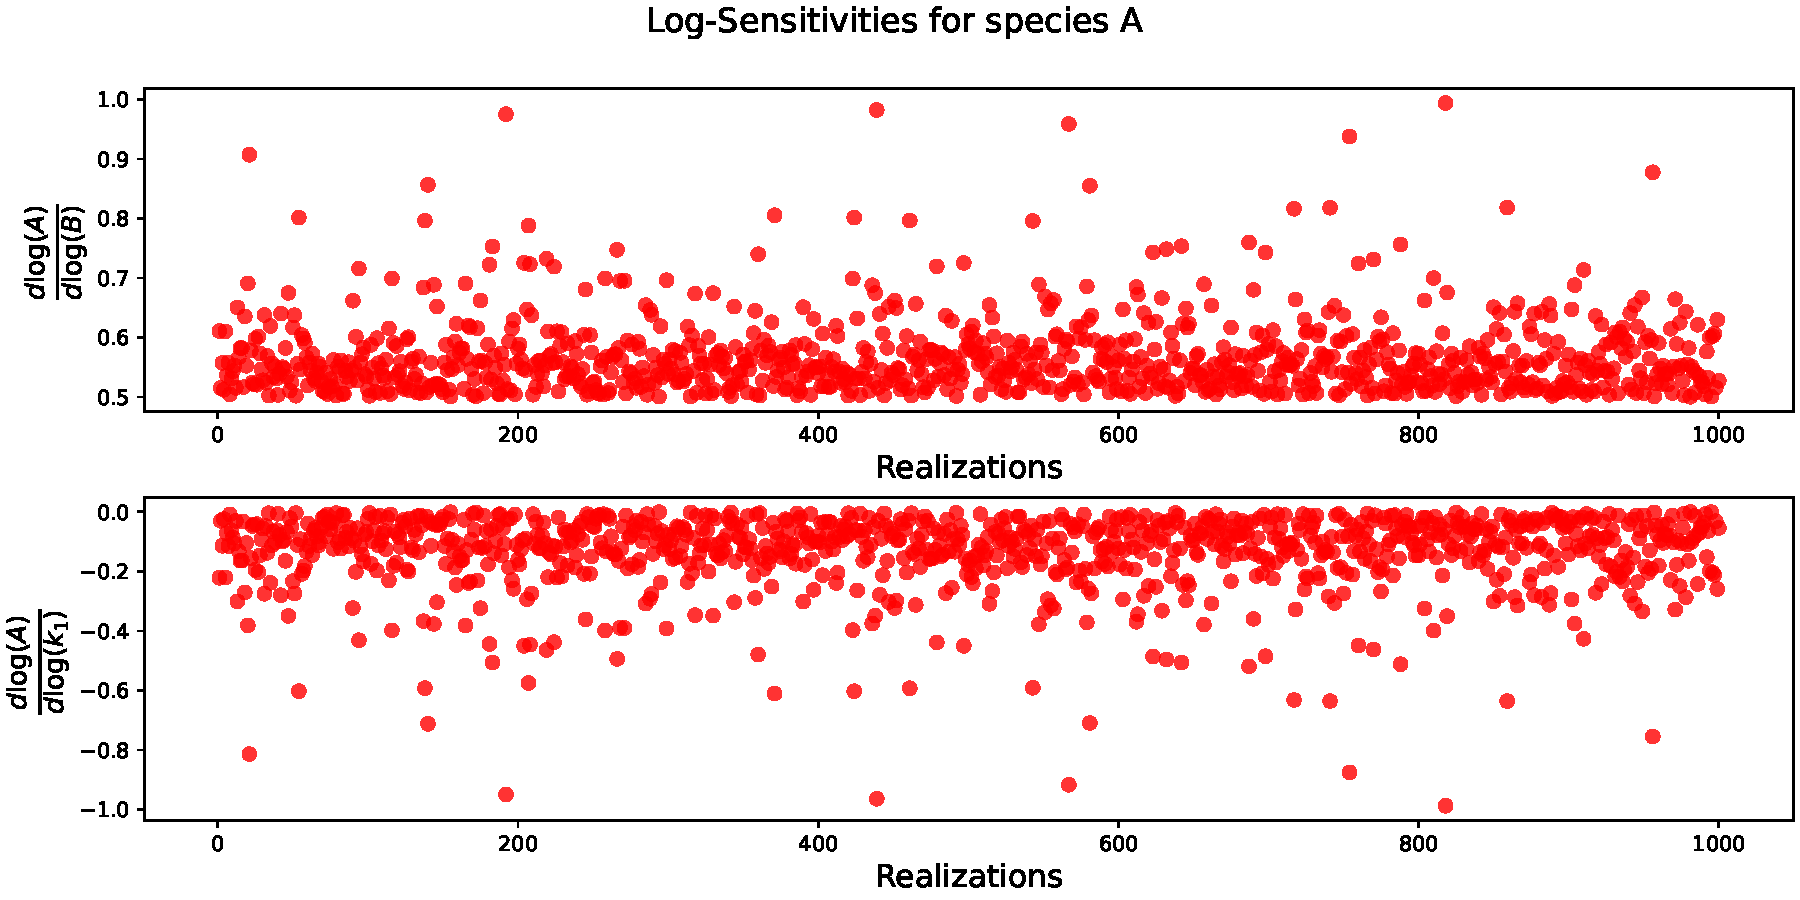
\includegraphics[width=1 \linewidth]{Sens_type1_chemoX2.pdf}
		\caption{\small{Numerical simulation for Type 1, with $\alpha = 1$ and $\beta = 2$ with 1000 realizations and randomized rate constants between 0 and 1. The results are only shown for perturbation on the chemostat and on $k_{-1}$. Log-sensitivities correctly follow the analytically predicted bounds, for B chemostated.}}
		\label{Fig. 2}
	\end{figure}
	
	
	\subsection{Sensitivities of type II network}
	
	We will analyze only the case in which A is chemostated:
	
	\begin{center}
		\begin{equation}
			\label{ex1}
			\newline
			\begin{aligned}
				\mathrm{A} &\xrightleftharpoons[j_{-1}]{j_{+1}}\mathrm{B}\\
				\mathrm{B} &\xrightleftharpoons[j_{-2}]{j_{+2}}\mathrm{C}\\
				\mathrm{C} &\xrightleftharpoons[j_{-1}]{j_{+1}}\mathrm{A}+\mathrm{B}
			\end{aligned}
		\end{equation}
	\end{center}
	
	Fixing the chemostat will fix the quantities
	
	\begin{center}
		\begin{equation}
			\begin{aligned}
				S = \begin{pmatrix}
					1 & -1 & 1 \\
					0 & 1 & -1
				\end{pmatrix} \quad \quad
				\mathbb{J}_{\mathbf{x}} = \begin{pmatrix}
					- k_{-1} & 0 \\
					k_{2} & -k_{-2} \\
					- k_{-3} a & k_3
				\end{pmatrix}
				\label{88}
			\end{aligned}
		\end{equation}
	\end{center}
	
	as well as
	
	\begin{center}
		\begin{equation}
			\begin{aligned}
				- (S \cdot  \mathbb{J}_{\mathbf{x}})^{-1} = \begin{pmatrix}
					\frac{1}{k_{-1}} & \frac{1}{k_{-1}} \\
					\frac{a k_{-3}+k_2}{k_{-1}(k_{-2}+k_3)} & \frac{a k_{-3}+k_2+k_{-1}}{k_{-1}(k_{-2}+k_3)}  
				\end{pmatrix}
				\label{89}
			\end{aligned}
		\end{equation}
	\end{center}
	
	Perturbing A one has 
	\begin{center}
		\begin{equation}
			\begin{aligned}
				\mathbf{J}_{a}= \begin{pmatrix}
					k_1\\
					0\\
					-k_{-3} b
				\end{pmatrix}
				\label{90}
			\end{aligned}
		\end{equation}
	\end{center}
	
	so that, following \eqref{11}:
	
	\begin{center}
		\begin{equation}
			\begin{aligned}
				\mathbf{x}_a= \begin{pmatrix}
					\frac{k_1}{k_{-1}} \\ \\
					\frac{2 a k_{-3} k_1 +k_1 k_2}{k_{-1}(k_{-2}+k_3)}
				\end{pmatrix}
				\label{91}
			\end{aligned}
		\end{equation}
	\end{center}
	
	Thus giving, exploiting the steady states
	
	
	\begin{center}
		\begin{equation}
			\begin{aligned}
				\frac{d \log b}{d \log a} &= 1 \\
				\frac{d \log c}{d \log a} &= \frac{2 k_{-3} a + k_2}{k_{-3} a + k_2} &\in \left[1, \right2]
			\end{aligned}
		\end{equation}
	\end{center}
	
	Perturbing $k_1$ one has
	
	\begin{center}
		\begin{equation}
			\begin{aligned}
				\mathbf{J}_{k_1}= \begin{pmatrix}
					a\\
					0\\
					0
				\end{pmatrix}
				\label{93}
			\end{aligned}
		\end{equation}
	\end{center}
	
	so that, following \eqref{11}:
	
	\begin{center}
		\begin{equation}
			\begin{aligned}
				\mathbf{x}_{k_1}= \begin{pmatrix}
					\frac{a}{k_{-1}} \\ \\
					\frac{a^2 k_{-3} +a k_2}{k_{-1}(k_{-2}+k_3)}
				\end{pmatrix}
				\label{94}
			\end{aligned}
		\end{equation}
	\end{center}
	
	
	Thus giving, exploiting the steady states
	
	\begin{center}
		\begin{equation}
			\begin{aligned}
				\frac{d \log b}{d \log k_1} &= \frac{k_1 a}{k_{-1} b} =1 \\
				\frac{d \log c}{d \log k_1} &= \frac{k_1}{c} \frac{a^2 k_{-3} +a k_2}{k_{-1}(k_{-2}+k_3)} = 1
			\end{aligned}
		\end{equation}
	\end{center}
	
	Perturbing $k_2$ one has
	
	\begin{center}
		\begin{equation}
			\begin{aligned}
				\mathbf{J}_{k_2}= \begin{pmatrix}
					0\\
					b\\
					0
				\end{pmatrix}
				\label{95}
			\end{aligned}
		\end{equation}
	\end{center}
	
	so that, following \eqref{11}:
	
	\begin{center}
		\begin{equation}
			\begin{aligned}
				\mathbf{x}_{k_2}= \begin{pmatrix}
					0 \\ \\
					\frac{k_1 b}{k_{-1}(k_{-2}+k_3)}
				\end{pmatrix}
				\label{96}
			\end{aligned}
		\end{equation}
	\end{center}
	
	
	Thus giving, exploiting the steady states
	
	\begin{center}
		\begin{equation}
			\begin{aligned}
				\frac{d \log b}{d \log k_2} &= 0 \\
				\frac{d \log c}{d \log k_2} &= \frac{k_2 }{a k_{-3} + k_2} \in \left[0, 1 \right]
			\end{aligned}
		\end{equation}
	\end{center}
	
	Perturbing $k_3$ one has
	
	\begin{center}
		\begin{equation}
			\begin{aligned}
				\mathbf{J}_{k_3}= \begin{pmatrix}
					0\\
					0\\
					c
				\end{pmatrix}
				\label{99}
			\end{aligned}
		\end{equation}
	\end{center}
	
	so that, following \eqref{11}:
	
	\begin{center}
		\begin{equation}
			\begin{aligned}
				\mathbf{x}_{k_3}= \begin{pmatrix}
					0 \\ \\
					-\frac{k_{-1}c}{k_{-1}(k_{-2}+k_3)}
				\end{pmatrix}
				\label{100}
			\end{aligned}
		\end{equation}
	\end{center}
	
	
	Thus giving, exploiting the steady states
	
	\begin{center}
		\begin{equation}
			\begin{aligned}
				\frac{d \log b}{d \log k_3} &= 0 \\
				\frac{d \log c}{d \log k_3} &= -\frac{k_{-1} k_3 }{k_{-1}k_{-2} + k_{-1}k_3} \in \left[-1, 0 \right]
			\end{aligned}
		\end{equation}
	\end{center}
	
	Perturbing $k_{-1}$ one has
	
	\begin{center}
		\begin{equation}
			\begin{aligned}
				\mathbf{J}_{k_{-1}}= \begin{pmatrix}
					-b\\
					0\\
					0
				\end{pmatrix}
				\label{102}
			\end{aligned}
		\end{equation}
	\end{center}
	
	so that, following \eqref{11}:
	
	\begin{center}
		\begin{equation}
			\begin{aligned}
				\mathbf{x}_{k_{-1}}= \begin{pmatrix}
					-\frac{b}{k_{-1}} \\ \\
					-\frac{k_{1}a (k_{-3}a +k_2)}{k_{-1}^2(k_{-2}+k_3)}
				\end{pmatrix}
				\label{103}
			\end{aligned}
		\end{equation}
	\end{center}
	
	
	Thus giving, exploiting the steady states
	
	\begin{center}
		\begin{equation}
			\begin{aligned}
				\frac{d \log b}{d \log k_{-1}} &= -1 \\
				\frac{d \log c}{d \log k_{-1}} &= -1
			\end{aligned}
		\end{equation}
	\end{center}
	
	Perturbing $k_{-2}$ one has
	
	\begin{center}
		\begin{equation}
			\begin{aligned}
				\mathbf{J}_{k_{-2}}= \begin{pmatrix}
					0\\
					-c\\
					0
				\end{pmatrix}
				\label{105}
			\end{aligned}
		\end{equation}
	\end{center}
	
	so that, following \eqref{11}:
	
	\begin{center}
		\begin{equation}
			\begin{aligned}
				\mathbf{x}_{k_{-2}}= \begin{pmatrix}
					0 \\ \\
					-\frac{c}{k_{-2}+k_3}
				\end{pmatrix}
				\label{106}
			\end{aligned}
		\end{equation}
	\end{center}
	
	
	Thus giving, exploiting the steady states
	
	\begin{center}
		\begin{equation}
			\begin{aligned}
				\frac{d \log b}{d \log k_{-2}} &= 0 \\
				\frac{d \log c}{d \log k_{-2}} &= \frac{k_{-3} a }{k_{-3} a + k_2} \in \left[0,1 \right]
			\end{aligned}
		\end{equation}
	\end{center}
	
	In conclusion, perturbing $k_{-3}$ one has
	
	\begin{center}
		\begin{equation}
			\begin{aligned}
				\mathbf{J}_{k_{-3}}= \begin{pmatrix}
					0\\
					0\\
					- a b
				\end{pmatrix}
				\label{108}
			\end{aligned}
		\end{equation}
	\end{center}
	
	and following \eqref{11}:
	
	\begin{center}
		\begin{equation}
			\begin{aligned}
				\mathbf{x}_{k_{-3}}= \begin{pmatrix}
					0 \\ \\
					-\frac{k_{1}a^2}{k_{-1}(k_{-2}+k_3)}
				\end{pmatrix}
				\label{100}
			\end{aligned}
		\end{equation}
	\end{center}
	
	
	Lastly giving
	
	\begin{center}
		\begin{equation}
			\begin{aligned}
				\frac{d \log b}{d \log k_{-3}} &= 0 \\
				\frac{d \log c}{d \log k_{-3}} &= \frac{k_{-3} a}{k_{-3} a +k_2} \in \left[0, 1 \right]
			\end{aligned}
		\end{equation}
	\end{center}
	
	\begin{figure}[H]
		\centering
		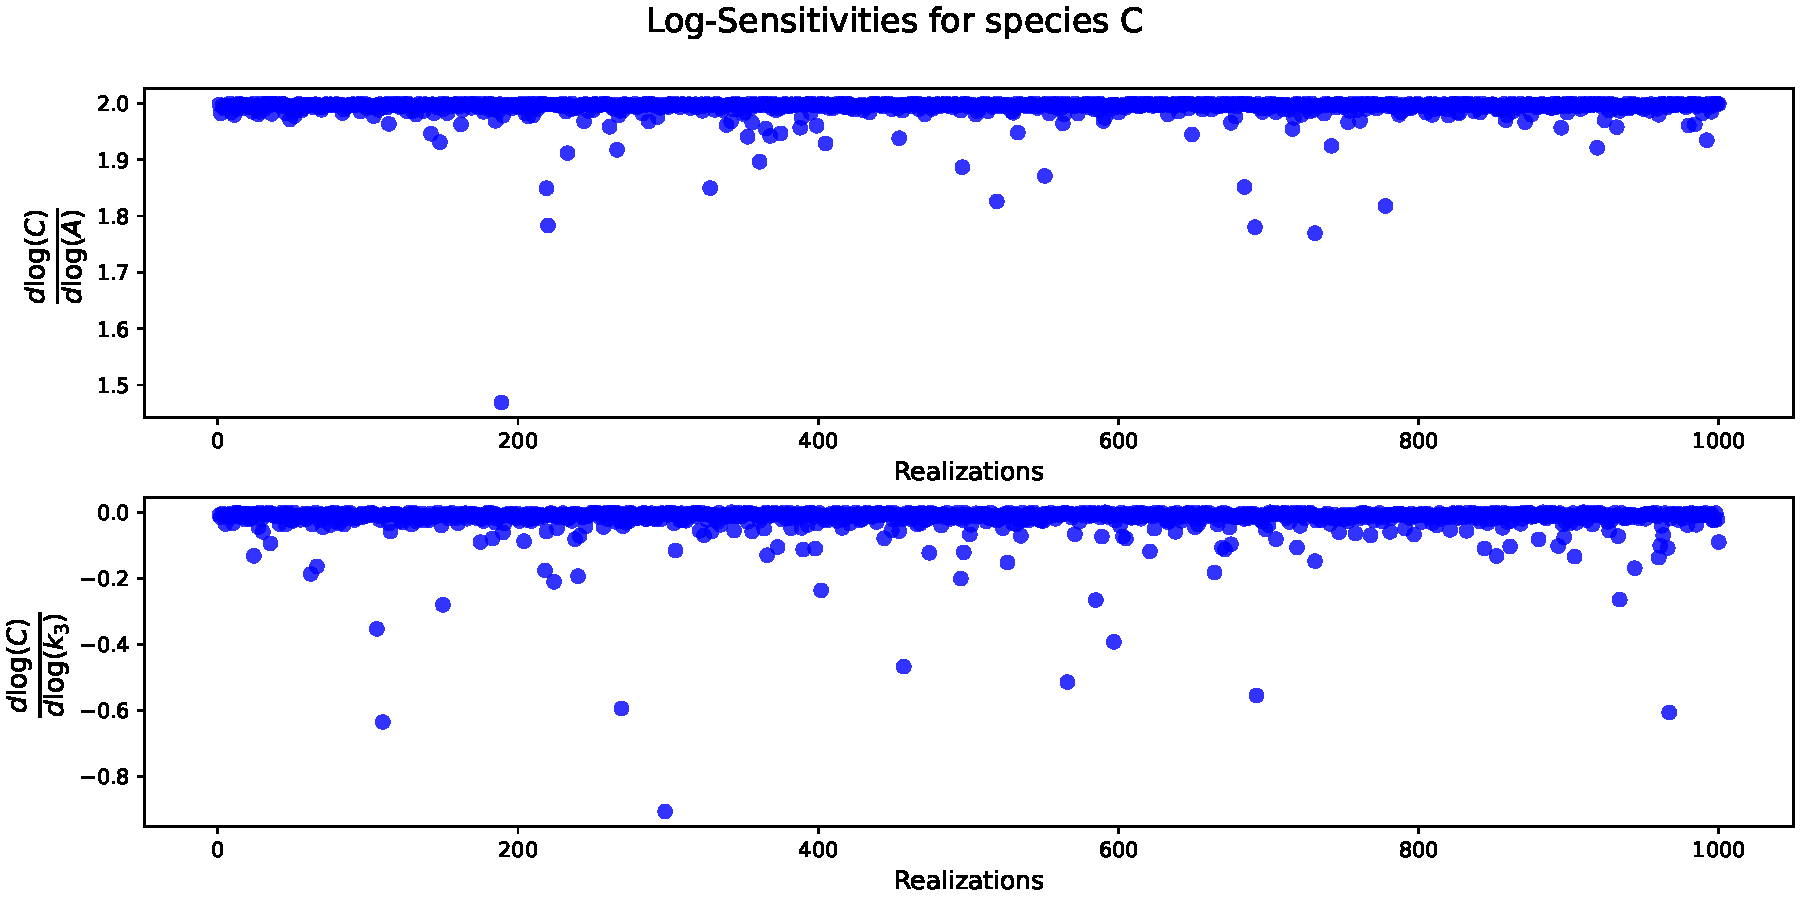
\includegraphics[width=0.95 \linewidth]{Sens_X3_chemoA.pdf}
		\caption{\small{Numerical simulation for Type 2 with 1000 realizations and randomized rate constants between 0 and 1. Responses of the concentration of species $C$ to different  parameters of the network. The results are only shown for perturbation with respect to the chemostat concentration $a$ and with respect to $k_{3}$. Log-sensitivities correctly follow the analytically predicted bounds, for A chemostated.}}
		\label{Fig. 4}
	\end{figure}
	
	The property $d \log b/ d \log k_{-3} =0$ means physically that $k_{-3}$ has no influence on the steady-concentration of $B$. This is expected since in the steady-state $b=k_1 a/k_{-1}$, which is a constant when $A$ is chemostated, independent of $k_{\pm 3}, k_{\pm 2}$. Thus, we see that zero sensitivity coefficients inform on the relative independence of parameters in the steady-state. 
	
	\section{Application to a system with conservation laws}
	
	We have noted before that \eqref{11} was just a particular case when there are no conserved quantities, so that $\mathbf{S} = \mathbf{S_R}$ is of maximum rank and the link matrix $\mathbf{L}$ is the identity matrix. We now study a case in which a conservation law is present in the network, such that the generalized \eqref{39} is needed.
	
	Let us consider again the Type 1 network of Eq. \ref{ex1}, but let us now assume that fuel $F$ and waste $W$ species are not anymore chemostated, while $A$ is.
	As a result, the stoichiometric matrix has now three rows corresponding to species $F$, $W$ and $B$ in that order :
	\begin{center}
		\begin{equation}
			\begin{aligned}
				\mathbf{S} = \begin{pmatrix}
					-1 & 0 \\
					0 & 1 \\
					1 & -1
				\end{pmatrix}.
			\end{aligned}
		\end{equation}
	\end{center}
	In this case, there is clearly a conserved quantity $l$ such that 
	\begin{center}
		\begin{equation}
			l \coloneqq f + w + b.
			\label{113}
		\end{equation}
	\end{center}
	
	Thus, a link matrix $\mathbf{L}$ should exist that links the stoichiometric matrix $\mathbf{S}$ to its reduced and full rank form $\mathbf{S_R}$ such that $\mathbf{S} = \mathbf{L} \cdot \mathbf{S_R}$. One possible choice is for instance :
	\begin{center}
		\begin{equation}
			\begin{aligned}
				\mathbf{L} = \begin{pmatrix}
					1 & 0 \\
					0 & 1 \\
					-1 & -1
				\end{pmatrix} \quad {\rm and} \quad
				\mathbf{S_R} = \begin{pmatrix}
					-1 & 0 \\
					0 & 1
				\end{pmatrix}.
			\end{aligned}
		\end{equation}
	\end{center}
	
	We can now look for the steady state by solving  $\mathbf{S_R} \cdot \mathbf{j} = 0$ together with the conservation law \eqref{113}.
	We find :
	\begin{center}
		\begin{equation}
			\begin{cases}
				\begin{aligned}
					l = f + w + b\\
					k_1 f a = k_{-1} b \\
					k_2 b = k_{-2} w a^2      
				\end{aligned}
			\end{cases}
			\label{115}
		\end{equation}
	\end{center}
	where we remind that $a$ is constant, since species $A$ is chemostated. Note that the system is reaching equilibrium even though $A$ is chemostated, because $F$ and $W$ are not chemostated anymore.
	The system \eqref{115} can be easily solved:
	
	\begin{center}
		\begin{equation}
			b &=\frac{a^2 k_{-2} k_1 l}{a k_{-2} \left(a k_1+k_{-1}\right)+k_1 k_2}
			\label{116}
		\end{equation}
		\begin{equation}
			f &=\frac{a k_{-2} k_{-1} l}{a k_{-2} \left(a k_1+k_{-1}\right)+k_1 k_2}
		\end{equation}
		\begin{equation}
			w &=\frac{k_1 k_2 l}{a k_{-2} \left(a k_1+k_{-1}\right)+k_1 k_2}
		\end{equation}
	\end{center}
	
	Now, to compute sensitivities with respect to every parameter, we recall equation \eqref{39}. We specify the external parameters as the vector
	
	\begin{center}
		\begin{equation}
			\pmb{\kappa} = \begin{pmatrix}
				k_1\\
				k_{-1}\\
				k_2\\
				k_{-2}\\
				a
			\end{pmatrix}
		\end{equation}
	\end{center}
	
	\begin{flushleft}
		Then, we still need to compute $\pmb{\bar{\epsilon}_{\kappa}}$, $\pmb{\bar{\epsilon}_{x}}$ and $\mathbf{M}$. The first two being
	\end{flushleft}
	
	\begin{center}
		\begin{equation}
			\pmb{\bar{\epsilon}_{\kappa}} = \begin{pmatrix}
				f a & -b & 0 & 0 & f k_1 \\
				0 & 0 & b & - w a^2 & -2wak_{-2}\\
			\end{pmatrix}
		\end{equation}
	\end{center}
	
	
	\begin{center}
		\begin{equation}
			\pmb{\bar{\epsilon}_{x}} = \begin{pmatrix}
				k_1 a & 0 & -k_{-1} \\
				0 & -k_{-2} a^2 & k_2 \\
			\end{pmatrix}
		\end{equation}
	\end{center}
	
	\begin{flushleft}
		So $\mathbf{M}$ can be constructed as
	\end{flushleft}
	
	\begin{center}
		\begin{equation}
			\mathbf{M} = \mathbf{S_R} \cdot \pmb{\bar{\epsilon}_{x}} \cdot \mathbf{L} =  \begin{pmatrix}
				-1 & 0 \\
				0 & 1
			\end{pmatrix}
			\begin{pmatrix}
				k_1 a & 0 & -k_{-1} \\
				0 & -k_{-2} a^2 & k_2 \\
			\end{pmatrix}
			\begin{pmatrix}
				1 & 0 \\
				0 & 1 \\
				-1 & -1
			\end{pmatrix} = \\
			= --
			\begin{pmatrix}
				k_1 a + k_{-1} & k_{-1} \\
				k_2 & k_{-2} a^2 + k_2 
			\end{pmatrix}
			
		\end{equation}
	\end{center}
	
	\begin{flushleft}
		So that 
	\end{flushleft}
	
	\begin{center}
		\begin{equation}
			- \mathbf{M}^{-1} = \frac{1}{k_1 k_{-2} a^3 + k_1 k_2 a + k_{-1} k_{-2} a^2} \begin{pmatrix}
				k_{-2}a^2 + k_2 & - k_{-1} \\
				- k_2 & k_1 a + k_{-1}
			\end{pmatrix}
		\end{equation}
	\end{center}
	
	\begin{flushleft}
		Now we have all the elements to construct equation \eqref{39}
	\end{flushleft}
	
	\begin{center}
		\begin{equation*}
			\frac{\partial \mathbf{x}}{\partial \pmb{\kappa}}
			= \mathbf{L} \cdot (-\mathbf{M}^{-1}) \cdot \mathbf{S_R} \cdot \bm{\Bar{\epsilon}_{\kappa}} =
		\end{equation}
	\end{center}
	
	\begin{center}
		\begin{equation*}
			= \frac{1}{\textrm{det($\mathbf{M}$)}} 
			\resizebox{0.9\textwidth}{!}{%
				
				\begin{pmatrix}
					-f a (k_{-2} a^2 + k_2) & b(k_{-2} a^2 + k_2) & -b k_{-1} & k_1 w a^2 & 2k_{-1}k_{-2} w a + f k_1 (k_{-2}a^2 + k_2) \\
					k_2 f a & -k_2 b & b(k_1 a +k_{-1}) & -wa^2(k_1 a +k_{-1} & f k_1 k_2 - 2 k_{-2}wa(k_1 a +k_{-1})\\
					k_{-2} f a^3 & -bk_{-2}a^2 & -b k_1 a & k_1 w a^3 & k_1 k_{-2} a^2 (f+2w)
			\end{pmatrix}}
		\end{equation}
	\end{center}
	
	\hfill \break
	We remind that the rows represent the response variable (respectively $f$, $w$, $b$) whereas the columns the perturbed parameter ($k_1$, $k_{-1}$, $k_2$, $k_{-2}$, $a$). For instance, we can study $\frac{\partial b}{\partial a}$ taking the third row and fifth column:
	
	\begin{center}
		\begin{equation}
			\frac{\partial b}{\partial a} = \frac{k_1 k_{-2} a^2 (f+2w)}{k_1 k_{-2} a^3 + k_1 k_2 a + k_{-1} k_{-2} a^2}
		\end{equation}
	\end{center}
	
	and the log-sensitivity, inserting $b$ from \eqref{116} gives
	
	\begin{center}
		\begin{equation}
			\frac{\partial \log b}{\partial \log a} &= \frac{a}{b} \frac{k_1 k_{-2} a (f+2w)}{k_1 k_{-2} a^2 + k_1 k_2 + k_{-1} k_{-2} a} = 
		\end{equation}
		\begin{equation}
			&=\frac{2 k_1 k_2 + k_1 k_{-2} a}{k_1 k_2 + k_1 k_{-2} a + k_1 k_{-2} a^2} \in \left[0, 2 \right]
		\end{equation}
	\end{center}
	
	Thus, we find that the sensitivity coefficient is 
	changed from Eq. \ref{eq:bound_A_chem} due to the conservation law. This is a result of having considered species $F$ and $W$ as internal and not anymore chemostated ones. In fact, previously, these 2 species had constant concentration and their effect could be absorbed in the rate constants. Now instead they are free to change during the dynamics, reaching a steady state through time and allowing a conservation law to show up. This means that even though the system looks quite similar to Type 1 with only $B$ as internal species, it actually differs from it, consequently giving different bounds for typical sensitivities.  
	
	\printbibliography
	
	\appendix
	
	\section*{Appendix A : MCA framework}
	
	Here, we recall some elements of Metabolic Control Analysis  \cite{3}, which are relevant for our subject. We start with the kinetic model :
	\begin{center}
		\begin{equation}
			\frac{d \mathbf{x}}{d t} = \mathbf{S} \cdot \mathbf{j} [\mathbf{x}, \pmb{\kappa}].
			\label{24}
		\end{equation}
	\end{center}
	where $\mathbf{x}$ is the vector of concentrations, $\mathbf{j}$ is the vector of currents, depending on the species themselves, $\mathbf{J}$ is the vector of steady state currents and external parameter $\mathbf{\kappa}$. In general, $\mathbf{S}$ is reducible because its rows are not independent due to conservation laws. In that case, one can introduce the following link matrix $\mathbf{L}$, such that $\mathbf{S}=\mathbf{L} \cdot \mathbf{S_R}$$.
	
	Considering $m$ species, $n$ reactions, $r$ the number of independent species (i.e. the rank of $\mathbf{S}$), $\mathbf{L}$ is a $m \times r$ matrix, and its rows can be arranged such that :
	\begin{center}
		\begin{equation}
			\mathbf{L}=\left[\begin{matrix}
				\mathbf{I}_r \\
				\mathbf{L_0}
			\end{matrix}\right] \ \ \ \ \ \ \  \mathbf{x}=\left[\begin{matrix}
				\mathbf{x_i} \\
				\mathbf{x_d}
			\end{matrix}\right]
		\end{equation}
	\end{center}
	where $\mathbf{x_i}$ (resp. $\mathbf{x_d}$) describe independent (resp. dependent) species. Then, we have 
	\begin{center}
		\begin{equation}
			\frac{d \mathbf{x}}{d t} = \mathbf{L} \cdot \frac{d \mathbf{x_i}}{d t}
			\label{27}
		\end{equation}
	\end{center}
	
	Similarly to the dependence between the rows of $\mathbf{S}$ which can be taken care of with the link matrix $\mathbf{L}$, the linear dependence between the columns of $\mathbf{S}$ can be taken care of with another matrix, the kernel matrix $\mathbf{K}$. This matrix allows to express steady-state fluxes $\mathbf{J}$ only in terms of independent ones $\mathbf{J}_i$. 
	\begin{center}
		\begin{equation}
			\mathbf{J} = \mathbf{K} \cdot \mathbf{J_i}
		\end{equation}
	\end{center}
	
	\subsection*{Elasticity matrices}
	In MCA, the derivatives of the fluxes are collected in elasticity matrices. Indeed, knowing $\mathbf{j} [\mathbf{x}, \pmb{\kappa}]$, we define the coefficient :
	\begin{center}
		\begin{equation}
			\Bar{\epsilon}^{j_k}_{x_i} = \frac{\partial j_k}{\partial x_i}, 
			\label{29}
		\end{equation}
	\end{center}
	which are coefficients of the matrix $\bm{\Bar{\epsilon}_x}$. The same can be done with respect to the set of parameters $\pmb{\kappa}$:
	\begin{center}
		\begin{equation}        \Bar{\epsilon}^{j_k}_{\kappa_i} = \frac{\partial j_k}{\partial \kappa_i}
			\label{30}
		\end{equation}
	\end{center}
	
	This will be the elasticity matrix $\bm{\Bar{\epsilon}_{\kappa}}$
	
	\subsection*{Perturbation with respect to an external parameter $\kappa$}
	We are interested in the system response, in terms of species concentrations and fluxes to a variation of the external parameter $\pmb{\kappa}$. From equation \eqref{24}, we start with the response of the independent variables at steady state:
	\begin{center}
		\begin{equation}
			\mathbf{S_R} \cdot \mathbf{j} [\mathbf{x}, \pmb{\kappa}] = \mathbf{0}
			\label{24}
		\end{equation}
	\end{center}
	
	\begin{flushleft}
		Differentiating with respect to $\pmb{\kappa}$
	\end{flushleft}
	
	\begin{center}
		\begin{equation}
			\mathbf{S_R} \left[\left( \frac{\partial \mathbf{j}}{\partial \mathbf{x_i}}\right)_{\mathbf{s_d,p}} \left( \frac{\partial \mathbf{x_i}}{\partial \pmb{\kappa}}\right) + \left( \frac{\partial \mathbf{j}}{\partial \mathbf{x_d}}\right)_{\mathbf{s_i,p}} \left( \frac{\partial \mathbf{x_d}}{\partial \mathbf{x_i}}\right)_{\pmb{\kappa}}\left( \frac{\partial \mathbf{x_i}}{\partial \pmb{\kappa}}\right)+ \left( \frac{\partial \mathbf{j}}{\partial \pmb{\kappa}}\right)\right] = \mathbf{0}
		\end{equation}
	\end{center}
	
	\begin{flushleft}
		Knowing, by solving \eqref{27}, that $\left( \frac{\partial \mathbf{x_d}}{\partial \mathbf{x_i}}\right)_{\pmb{\kappa}}=\mathbf{L_0}$, we can insert this to find
	\end{flushleft}
	
	\begin{center}
		\begin{equation}
			\mathbf{S_R} \bigg{\left[ \begin{matrix}
					\frac{\partial \mathbf{j}}{\partial \mathbf{x_i}} &
					\frac{\partial \mathbf{j}}{\partial \mathbf{x_d}}
				\end{matrix}\right]}
			\left[ \begin{matrix}
				\mathbf{I}_r \\
				\mathbf{L_0}
			\end{matrix}\right]
			\left( \frac{\partial \mathbf{x_i}}{\partial \pmb{\kappa}}\right)+\mathbf{S_R}\left( \frac{\partial \mathbf{j}}{\partial \pmb{\kappa}}\right) = \mathbf{0}
		\end{equation}
	\end{center}
	
	\begin{flushleft}
		and we recognize the elasticity matrices, thanks to definitions \eqref{29} and \eqref{30}:
	\end{flushleft}
	
	\begin{center}
		\begin{equation}
			\mathbf{S_R} \cdot \bm{\Bar{\epsilon}_x} \cdot \mathbf{L}
			\cdot \frac{\partial \mathbf{x_i}}{\partial \pmb{\kappa}}
			+ \mathbf{S_R} \cdot \bm{\Bar{\epsilon}_{\kappa}} = \mathbf{0}
			\label{34}
		\end{equation}
	\end{center}
	
	\begin{flushleft}
		A similar relation can be derived for the steady state fluxes, being already explicit:
	\end{flushleft}
	
	\begin{center}
		\begin{equation}
			\frac{\partial \mathbf{J}}{\partial \pmb{\kappa}}=\bm{\Bar{\epsilon}_x} \cdot \mathbf{L} \cdot 
			\frac{\partial \mathbf{x_i}}{\partial \pmb{\kappa}}+\bm{\Bar{\epsilon}_{\kappa}}
		\end{equation}
	\end{center}
	
	Since we're interested in the \textbf{concentration response with respect to $\kappa$}, we focus on equation \eqref{34}. In fact, the product
	
	\begin{center}
		\begin{equation}
			\mathbf{S_R} \cdot \bm{\Bar{\epsilon}_x} \cdot \mathbf{L} \coloneqq \mathbf{M}
		\end{equation}
	\end{center}
	
	\begin{flushleft}
		is what we usually call Jacobian of the system, generalized to the case in which this shows conservation laws. \textbf{It has been proven that if a steady state exists, the Jacobian $\mathbf{M}$ will be invertible, but its individual product elements will not necessary be}. This means we can explicit the concentration response with respect to parameters $\pmb{\kappa}$ from \eqref{34}:
	\end{flushleft}
	
	\begin{center}
		\begin{equation}
			\frac{\partial \mathbf{x_i}}{\partial \pmb{\kappa}}
			= -\mathbf{M}^{-1} \cdot \mathbf{S_R} \cdot \bm{\Bar{\epsilon}_{\kappa}}
		\end{equation}
	\end{center}
	
	and since 
	
	\begin{center}
		\begin{equation}
			\frac{\partial \mathbf{x_d}}{\partial \pmb{\kappa}}= \mathbf{L_0} \cdot \frac{\partial \mathbf{x_i}}{\partial \pmb{\kappa}}
			\label{38}
		\end{equation}
	\end{center}
	
	We find the general concentration sensitivity as 
	
	\begin{center}
		\begin{equation}
			\frac{\partial \mathbf{x}}{\partial \pmb{\kappa}}
			= -(\mathbf{L} \cdot \mathbf{M}^{-1} \cdot \mathbf{S_R}) \cdot \bm{\Bar{\epsilon}_{\kappa}}
			\label{39}
		\end{equation}
	\end{center}
	
	\begin{comment}
		Note that on the right-hand side, only $\bm{\Bar{\epsilon}_{\kappa}}$ depends explicitly on $\pmb{\kappa}$. One would then want to extract the elements of the matrix 
		
		\begin{center}
			\begin{equation}
				-(\mathbf{L} \mathbf{M}^{-1}\mathbf{S_R})=-(\mathbf{L} (\mathbf{S_R} \bm{\Bar{\epsilon}_x} \mathbf{L})^{-1}\mathbf{S_R})
			\end{equation}
		\end{center}
		
		This means we can extract the information about this matrix only if $\bm{\Bar{\epsilon}_{\kappa}}$ is invertible. Now, consider a set of parameters such that each uniquely affects a single
		reaction, i.e., in the elasticity matrix $\bm{\Bar{\epsilon}_{\kappa}}$
		
		\begin{center}
			\begin{equation}
				\frac{\partial j_i}{\partial \kappa_i} \neq 0 \ \ \textrm{and} \ \ \frac{\partial j_i}{\partial \kappa_l} =  0 \ \ \textrm{for} \ \ i \neq l
			\end{equation}
		\end{center}
		
		This will produce a diagonal $\bm{\Bar{\epsilon}_{\kappa}}$ so that we can define, on the left-hand side a \textbf{concentration-control coefficient}
		
		\begin{center}
			\begin{equation}
				\mathbf{\Bar{C}^s} = -\mathbf{L} \mathbf{M}^{-1}\mathbf{S_R}
			\end{equation}
		\end{center}
		
		with parameter-dependent elements
		
		\begin{center}
			\begin{equation}
				\Bar{C}^{x_j}_i = \frac{\partial x_j}{\partial \kappa_i} / \frac{\partial j_i}{\partial \kappa_i}
			\end{equation}
		\end{center}
		
	\end{comment}
	
	
	\printbibliography
	
\end{document}



-------------------
\subsection{Michaelis Menten for type 1}
We will now consider the rate law to be of the Michaelis-Menten type. Since this is analytically heavy, we will at first assume to have MM only for the forward rate of the first reaction, hence:

\begin{center}
	\begin{equation}
		\begin{aligned}
			J_{1} = \frac{a^{\alpha}}{k_1+a^{\alpha}} - k_{-1} b \\
			J_{2} = k_2 b - k_{-2} a^{\beta} 
		\end{aligned}
	\end{equation}
\end{center}

The calculations for this case are not trivial and redundant. In the following we'll show the results that one finds, when A is chemostated.


\begin{equation}
	\begin{aligned}
		\frac{d \log b}{d \log a} &\le \beta \\
		\frac{d \log b}{d \log k_1} &\in \left[ -1, 0 \right] \quad \textrm{(to be confirmed)} \\
		\frac{d \log b}{d \log k_2} &\in \left[ -1, 0 \right] \\
		\frac{d \log b}{d \log k_{-1}} &\in \left[ -1, 0 \right] \\
		\frac{d \log b}{d \log k_{-2}} &\in \left[ 0, 1 \right] \\
	\end{aligned}
\end{equation}
\\
Different instead is the case of having irreversible reaction, considering only the forward rates:

\begin{center}
	\begin{equation}
		\begin{aligned}
			J_{1} &= \frac{a^{\alpha}}{k_1+a^{\alpha}} \\
			J_{2} &= \frac{b}{k_2+b}
		\end{aligned}
	\end{equation}
\end{center}

In this case, any information on $\beta$ will be obviously lost. When A is chemostated for instance, and we perturb the concentration of A, one has:

\begin{center}
	\begin{equation}
		\begin{aligned}
			\mathbb{J}_b =  \begin{pmatrix}
				0 \\ \\
				\frac{k_2}{k_2 + b}
			\end{pmatrix} \quad \quad
			\mathbf{J}_{a} = \begin{pmatrix}
				\frac{\alpha k_1 a^{\alpha -1}}{(k_1 + a^{\alpha})^2} \\ \\
				0
			\end{pmatrix}
		\end{aligned}
	\end{equation}
\end{center}

which means

\begin{center}
	\begin{equation}
		\begin{aligned}
			S \cdot \mathbb{J}_b =  - \frac{k_2}{(k_2+b)^2} \quad \quad
			S \cdot \mathbf{J}_{a} = \frac{\alpha k_1 a^{\alpha -1}}{(k_1 + a^{\alpha})^2}
		\end{aligned}
	\end{equation}
\end{center}

which easily lead to an equality:

\begin{center}
	\begin{equation}
		\frac{d \log b}{d \log a} &= \alpha
	\end{equation}
\end{center}

For the rate constants, again, here we sum up the results obtained with the same method:

\begin{equation}
	\begin{aligned}
		\frac{d \log b}{d \log k_1} &= -1 \\
		\frac{d \log b}{d \log k_2} &= 1 
	\end{aligned}
\end{equation}

------------
\begin{figure}[H]
	\centering
	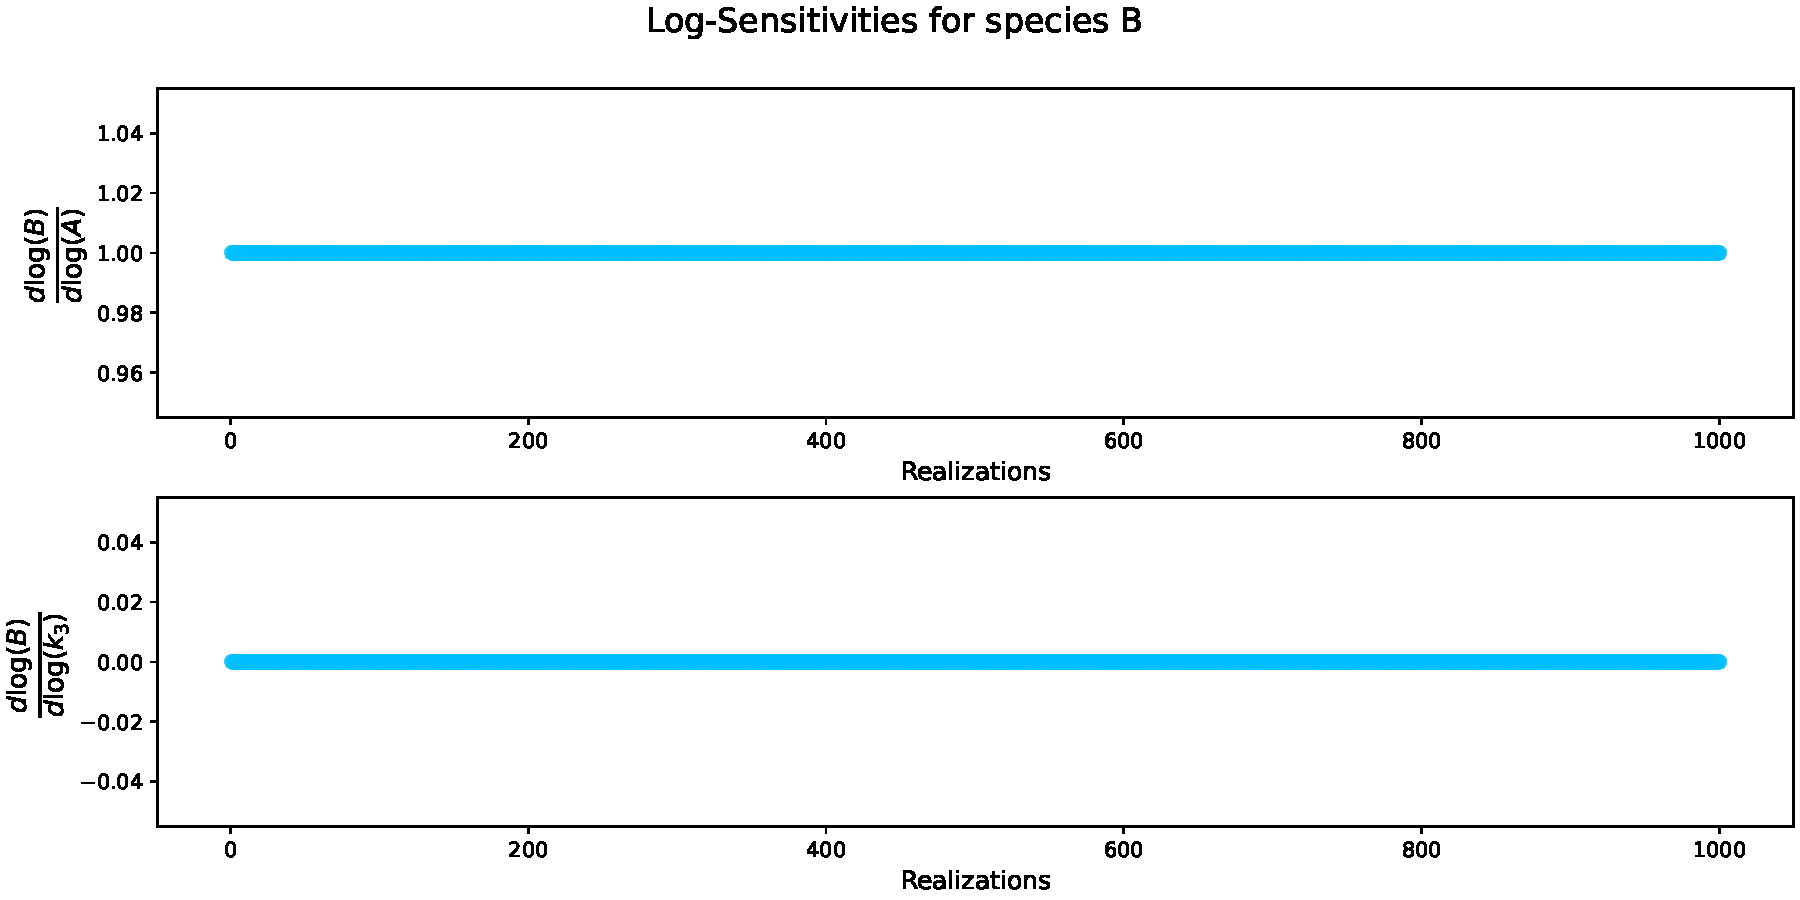
\includegraphics[width=1 \linewidth]{Sens_X2_chemoA.pdf}
	\caption{\small{Numerical simulation for Type 2 with 1000 realizations and randomized rate constants between 0 and 1. Responses of species B from perturbations of different parameters of the network. The results are only shown for perturbation on the chemostat and on $k_{3}$. Log-sensitivities correctly follow the analytically predicted bounds, for A chemostated.}}
	\label{Fig. 3}
\end{figure}
\\